% =====================================================================
% Paper 2 — When Hyperparameter-Free Decoding Silently Breaks:
% Looping of p-less Sampling in Reasoning-Model Code Generation
%
% Arc: failure -> mechanism -> G_k (Renyi-order) lever + ablation -> positioning.
% Every number traces to: docs/decoder_comparison_cot_apps_{deepseek,qwen3}.md and
% results/_renyi_sweep_full252/<model>/ATCODER_interview/analysis/pass_at_k_ablation_{qwen,deepseek}.md.
% Generic article class (compiles anywhere incl. Overleaf); [ICLR-SWAP] marks the documentclass to
% replace with iclr2027_conference.sty at submission.
% =====================================================================
\documentclass[11pt]{article}                       % [ICLR-SWAP]
\usepackage[margin=1in]{geometry}                    % [ICLR-SWAP]
\usepackage[utf8]{inputenc}
\usepackage{amsmath,amssymb}
\usepackage{booktabs}
\usepackage{graphicx}
\usepackage{float}   % [H] to pin appendix tables under their own section (no float pile-up)
\usepackage{multirow}
\usepackage[numbers]{natbib}
\usepackage[hidelinks]{hyperref}
\usepackage{xcolor}
\newcommand{\td}[1]{\textcolor{red}{[TODO: #1]}}
\newcommand{\tsum}{\ensuremath{\textstyle\sum}}
\graphicspath{{figures/}}

\title{When a Hyperparameter-Free Decoder Fails:\\
Diagnosing and Repairing p-less Sampling Loops\\ in Reasoning-Model Code Generation}
\author{}
\date{}

\begin{document}
\maketitle

\begin{abstract}
Hyperparameter-free decoders such as p-less sampling promise to remove temperature and top-$p$ tuning
by deriving a truncation threshold---the collision probability $\tsum_i p_i^2$ (R\'enyi order
$k{=}2$)---directly from the token distribution. We show this fails silently on reasoning models
generating code. On APPS (a competitive-programming code benchmark), two 8B reasoning models
(DeepSeek-R1-Distill, Qwen3) under default p-less send 14--42\% of chain-of-thought traces into
non-terminating loops---among the worst pass@1 of any decoder we test---at temperature $1.0$, where
temperature sampling does not loop. We trace this to a decoder-side mechanism: on the peaked
distributions of long reasoning, the collision threshold rises to meet the top token, collapsing the
survivor set to a single token and re-deriving the same step. The origin paper's appendix proposes generalizing the
threshold to any R\'enyi order $k$ ($G_k{=}\exp(-H_k)$) but evaluates only $k{=}2$; we give, to our
knowledge, the \emph{first empirical evaluation} at $k\neq2$ and find that \emph{lowering} $k$ escapes
the loops and recovers
accuracy---the best pass@1 on Qwen (beating even a hand-swept temperature), and a
calibration-free repair of a catastrophic default on DeepSeek.
\end{abstract}

\section{Introduction}\label{sec:intro}
Hyperparameter-free decoders are appealing because they remove the temperature/top-$p$/top-$k$ tuning
that otherwise depends on the model, task, and desired diversity. \citet{tan2025pless} propose
\textbf{p-less} and \textbf{p-less-norm}, truncation samplers whose admission threshold is the
collision probability $\tsum_i p_i^2$ of the distribution, with no tunable knobs, and evaluate them on
math, reasoning, and creative writing. We ask what happens on reasoning models generating
code---a setting the origin paper does not study, and one where the long, low-entropy thinking phase
stresses any decoder.

We find that p-less \emph{fails silently} there. On APPS with two 8B reasoning models, default p-less
sends 14--42\% of chain-of-thought traces into non-terminating loops that run to the token cap,
producing among the worst pass@1 of any decoder we test---while emitting no error and, at first glance,
no obvious pathology. Our contributions:
\begin{enumerate}\itemsep2pt
  \item \textbf{The silent failure} (\S\ref{sec:failure}): default p-less loops on reasoning-model
    code CoT, at temperature $1.0$, where temperature sampling does not.
  \item \textbf{A decoder-side mechanism} (\S\ref{sec:mech}): on peaked distributions the collision
    threshold meets the top probability, collapsing the survivor set to the single most-probable
    token exactly where the model is most confident.
  \item \textbf{The R\'enyi-order-$k$ lever, and why it works} (\S\ref{sec:alpha}): the origin paper's
    appendix proposes generalizing the threshold to any R\'enyi order $k$ ($G_k{=}\exp(-H_k)$) but
    evaluates only the default $k{=}2$; we give, to our knowledge, the \emph{first empirical evaluation}
    at $k\neq2$. Lowering $k$ removes loops, recovers accuracy, and cuts wasted thinking tokens. A
    per-problem ablation attributes the recovery to loop-escape---concentrated on \emph{borderline}
    problems (not a rich-get-richer effect) and at least $\sim$22\% non-loop on Qwen under a truncation bound.
  \item \textbf{Positioning} (\S\ref{sec:pos}): the optimal $k$ is model-dependent (Qwen $k{\approx}0.1$,
    DeepSeek $k{\approx}0.4$); $G_k$ has the best pass@1 on Qwen---beating even a hand-swept
    temperature---and a calibration-free repair that competes with, but does not beat, tuned temperature
    on DeepSeek.
\end{enumerate}
The value of a hyperparameter-free default is that it works out of the box; our point is that this one
silently does not, on an increasingly common setting, and that a single order parameter both explains
and repairs the failure.

\section{Background and Related Work}\label{sec:bg}
\paragraph{p-less and p-less-norm.} Given a distribution $p$ over a vocabulary of size $v$, p-less
admits tokens with $p_i \ge \tsum_j p_j^2$; p-less-norm relaxes the threshold to
$(v\tsum_j p_j^2 - 1)/(v-1)$. Survivors are renormalized and sampled; the only optional control is a
pre-truncation temperature~\citep{tan2025pless}.

\paragraph{Reasoning-model looping.} \citet{pipis2025loop} show reasoning models loop at low
temperature, attributing it to risk aversion---a \emph{model-side} propensity we cite rather than
claim. \citet{duan2026circular} characterize self-reinforcing loops as semantically redundant yet
lexically distinct and predict them from hidden-state transitions; \citet{xie2025wordsalad} note
reasoning models ``do not exhibit strictly verbatim repetitions'' and catch the resulting text with a
hidden-state probe. \citet{yang2025recover} show models identify but fail to recover from unhelpful
thoughts, with inverse scaling; DEER~\citep{yang2025deer} and s1~\citep{muennighoff2025s1} control
reasoning length reactively or by budget forcing. \textbf{All of this work is on math/QA and is
detection- or length-focused}: none evaluates code, and none studies a truncation sampler as a
\emph{cause} or \emph{preventive} of looping---the gaps we fill.

\paragraph{Truncation and degeneration.} \citet{holtzman2020curious} established that
likelihood-maximizing decoding produces repetitive, degenerate text; min-$p$
\citep{nguyen2024minp}, top-$n\sigma$~\citep{tang2024topnsigma}, and $\eta$-sampling
\citep{hewitt2022truncation} are knobbed truncation samplers. Our mechanism (\S\ref{sec:mech}) can be
seen as a truncation-sampler instance of that effect: because $\tsum_i p_i^2 \le \max_i p_i$, on
peaked steps the p-less threshold can admit only the most-probable token, so a purely
distribution-derived cutoff reproduces the repetition that maximization-based decoding is known to cause.

\section{Setup}\label{sec:setup}
\paragraph{Models, data, decoders.} We use DeepSeek-R1-Distill-Llama-8B~\citep{deepseekai2025r1} and
Qwen3-8B~\citep{yang2025qwen3} on 252 APPS ``interview'' problems~\citep{hendrycks2021apps}\footnote{APPS
interview split; problems executed against hidden tests.}, thinking enabled, 10 samples/problem,
generation capped at $32{,}768$ tokens. We
compare default p-less ($k{=}2$), p-less-norm, a R\'enyi-order sweep $G_k$ ($k$ from $1.6$ down to
$0.05$), temperature / top-$p$ / top-$k$ configurations including each model's officially recommended
setting, and an adaptive detect-and-chop rescue.

\paragraph{Metrics.} pass@1/@10 with the unbiased estimator of \citet{chen2021humaneval};
\emph{non-termination rate} (fraction of samples that never close the thinking phase within the token
budget---our loop proxy); self-CodeBLEU output diversity (\emph{cb\_div}; defined below); and mean
thinking tokens. Mean tokens count truncated samples at their cut length, so they are biased upward for
high-truncation configs---which is exactly the wasted-budget cost we want to expose.

\paragraph{Diversity via self-CodeBLEU.} We measure output diversity \emph{within} each
configuration's own samples, following the self-similarity principle of Self-BLEU~\citep{zhu2018texygen}:
a generator is diverse to the extent its samples differ from \emph{one another}, with no external
reference. For each problem we take the samples that pass the hidden tests, deduplicate structurally
identical ones by AST fingerprint, compute CodeBLEU~\citep{ren2020codebleu} for every unordered pair,
and report $\mathrm{cb\_div}=1-\overline{\mathrm{CodeBLEU}}$; the tabulated cb\_div is the mean over
problems with $\ge 2$ correct solutions. Higher is more diverse---we invert the similarity so cb\_div
reads in the same direction as pass@$k$ (Self-BLEU is conventionally lower-is-more-diverse). We use
CodeBLEU rather than token BLEU because it augments $n$-gram overlap with keyword-weighted $n$-grams,
abstract-syntax-tree matching, and data-flow matching (a weighted mean, default weights $0.25$ each),
so two solutions that differ only in variable names or formatting but share structure and data flow are
scored as similar rather than spuriously diverse---the appropriate notion for \emph{algorithmic}
diversity. Scoring only correct samples means cb\_div reflects diversity among \emph{working} solutions;
since each configuration is scored on its own correct subset, cross-configuration comparison carries a
mild confound (configurations with fewer correct solutions per problem contribute fewer pairs), which
we flag where it matters.

\paragraph{The R\'enyi-order-$k$ family.} We generalize the p-less threshold along the R\'enyi order
$k$ using the origin paper's own proposal, $G_k=\exp(-H_k)=(\tsum_i p_i^k)^{1/(k-1)}$
(Appendix~B.5 of \citet{tan2025pless}), where $H_k$ is the R\'enyi entropy of order $k$~\citep{renyi1961measures};
$k{=}2$ recovers default p-less (the collision threshold $\tsum_i p_i^2$). We sweep
$k\in\{1.6,0.8,0.4,0.2,0.1,0.05\}$; \emph{lowering} $k$ below $2$ loosens the filter (the threshold
drops, admitting more tail tokens). The origin paper proposes $G_k$ only theoretically---it analyzes
the asymptotics ($G_k\!\to\!1/v$ as $k\!\to\!0$, $G_k\!\to\!\max_i p_i$ as $k\!\to\!\infty$) and reports
no experiments at $k\neq2$---so our sweep is its first empirical evaluation.

\section{The silent failure}\label{sec:failure}
Table~\ref{tab:main} reports the full decoder comparison. Default p-less ($k{=}2$) and
p-less-norm are the worst configurations on DeepSeek (pass@1 $0.392$ vs.\ $0.480$ for the best
temperature) and among the worst on Qwen ($0.625$), driven by \textbf{non-termination rates of 41.8\%
(DeepSeek) and 14.5\% (Qwen)}: nearly half of DeepSeek's reasoning traces loop until the token cap.

\begin{figure}[t]\centering
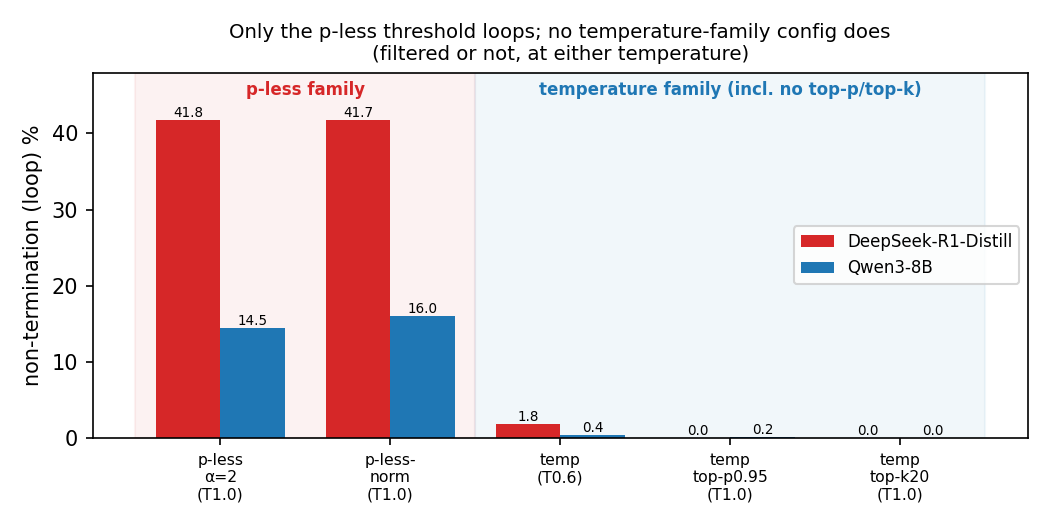
\includegraphics[width=0.62\linewidth]{fig_failure_t1.png}
\caption{Non-termination (loop) rate by decoder (per-bar temperature labeled). Default p-less and
p-less-norm loop on 14--42\% of traces; every temperature-family config loops far less ($\le$6.5\%),
and temperature with no top-$p$/top-$k$ stays near 0\%. The failure is thus specific to the
p-less threshold---not a low-temperature effect (p-less at $T{=}1.0$ still loops) and not the secondary
top-$p$/top-$k$ truncation (removing it does not induce looping).}
\label{fig:failuret1}
\end{figure}

The failure is easy to misattribute. Reasoning models are known to loop at low
temperature~\citep{pipis2025loop}, so one might dismiss this as the same effect, or attribute the
temperature configs' stability to their top-$p$/top-$k$ truncation. Figure~\ref{fig:failuret1} rules
out both: p-less loops on 14--42\% of traces \emph{at temperature $1.0$}, while every
temperature-family config loops far less ($\le$6.5\%; temperature with no top-$p$/top-$k$ at
1.8\% DeepSeek, 0.4\% Qwen). At a matched temperature the contrast is direct: on Qwen
at $T{=}0.6$, p-less loops on 19.0\% of traces versus 0.4\% for plain temperature. The pathology is
therefore \emph{structural to the p-less threshold}---neither a low-temperature effect nor a
consequence of secondary truncation---and it is silent: no crash, no warning, just a slow decline into
repetition that consumes the entire token budget.

\begin{table}[t]\centering\small
\caption{APPS decoder comparison (252 tasks, $n{=}10$, thinking on). Regenerated live; pass@$k$
cross-verified against stored values. \textbf{Bold} marks the best value per column among the
\emph{zero-tuning} configurations---defaults, the $G_k$ sweep ($k{=}2$ is default p-less), and each
model's officially recommended setting (``rec''). $^\dagger$ marks the strongest temperature found by
\emph{sweeping} $T$, a tuned reference (not eligible for bold). Lowering $k$ from the default removes
looping and recovers accuracy on both models: on Qwen, $G_k{=}0.1$ has the best pass@1 and pass@10 among
the zero-tuning configs (the tuned pure-temperature reference $^\dagger$ edges it on pass@10; App~\ref{app:topp});
on DeepSeek, $G_k$ leads on pass@10 / tokens / non-termination but trails the recommended temperature on
pass@1 by $0.006$. cb\_div is correct-only
and not ranked across configs (see \S\ref{sec:setup}). Full pass@$k$ and cover@$t$ in App~\ref{app:passk}.}
\label{tab:main}
\begin{tabular}{lccccc}
\toprule
Config & pass@1 & pass@10 & cb\_div & mean think tok & non-term \% \\
\midrule
\multicolumn{6}{l}{\textit{DeepSeek-R1-Distill-Llama-8B}}\\
p-less $k{=}2$ (default) & 0.392 & 0.627 & 0.489 & 17{,}269 & 41.8 \\
p-less-norm (default)    & 0.392 & 0.663 & 0.494 & 17{,}116 & 41.7 \\
$G_k{=}1.6$              & 0.400 & 0.643 & 0.494 & 16{,}420 & 39.6 \\
$G_k{=}0.8$              & 0.435 & 0.687 & 0.518 & 12{,}925 & 25.8 \\
$G_k{=}0.4$              & 0.469 & \textbf{0.730} & 0.575 & \textbf{9{,}615} & \textbf{0.0} \\
$G_k{=}0.2$              & 0.463 & \textbf{0.730} & 0.583 & 9{,}879 & \textbf{0.0} \\
$G_k{=}0.1$              & 0.463 & 0.714 & 0.588 & 9{,}994 & 0.2 \\
$G_k{=}0.05$            & 0.459 & 0.710 & 0.586 & 9{,}988 & \textbf{0.0} \\
temp $T{=}0.6,p0.95$ (rec)    & \textbf{0.475} & 0.714 & 0.534 & 9{,}866 & 6.2 \\
temp $T{=}1.0,p0.95$ $^\dagger$ & 0.480 & 0.726 & 0.556 & 9{,}683 & 0.0 \\
\midrule
\multicolumn{6}{l}{\textit{Qwen3-8B}}\\
p-less $k{=}2$ (default) & 0.625 & 0.825 & 0.453 & 13{,}485 & 14.5 \\
p-less-norm (default)    & 0.629 & 0.829 & 0.458 & 13{,}573 & 16.0 \\
$G_k{=}1.6$              & 0.627 & 0.813 & 0.464 & 12{,}971 & 14.0 \\
$G_k{=}0.8$              & 0.669 & 0.837 & 0.461 & 11{,}788 & 8.0 \\
$G_k{=}0.4$              & 0.696 & 0.833 & 0.457 & 10{,}912 & 0.4 \\
$G_k{=}0.2$              & 0.701 & 0.833 & 0.493 & 11{,}062 & \textbf{0.0} \\
$G_k{=}0.1$              & \textbf{0.719} & \textbf{0.845} & 0.498 & 10{,}808 & \textbf{0.0} \\
$G_k{=}0.05$            & 0.717 & 0.833 & 0.497 & \textbf{10{,}767} & 0.1 \\
temp $T{=}0.6,p0.95,k20$ (rec) & 0.680 & 0.829 & 0.468 & 11{,}127 & 1.0 \\
temp $T{=}1.0$ (unfilt) $^\dagger$ & 0.712 & 0.849 & 0.503 & 10{,}738 & 0.0 \\
\bottomrule
\end{tabular}
\end{table}

\section{The mechanism}\label{sec:mech}
Why does a truncation rule cause looping? Because the p-less threshold $\tsum_i p_i^2$ is bounded above
by the top probability, $\tsum_i p_i^2 \le \max_i p_i$, with equality approached as the distribution
concentrates. On the peaked next-token distributions typical of a confident reasoning step, the
threshold rises toward the mode and the survivor set can collapse to the single most-probable
token---on such steps p-less emits the argmax. Repeatedly emitting the argmax re-derives the same
continuation, and the model re-enters the same reasoning move---a loop. We do not measure the per-step
survivor count directly, but the controlled comparison of Figure~\ref{fig:failuret1}---p-less loops at
a matched temperature where plain sampling does not---is consistent with this collapse driving the
loop. This inverts the usual reading of truncation as a cure for repetition~\citep{holtzman2020curious}:
pinned to the collision probability, the threshold \emph{amplifies} repetition where the model is confident.

\paragraph{The loop is a joint effect, not a p-less artifact alone.} Self-reinforcing loops are a
documented \emph{model-side} phenomenon in reasoning models: \citet{pipis2025loop} attribute them to
risk aversion and temporally-correlated errors arising in training (not to the decoder), and
\citet{duan2026circular} study them as an internal, self-reinforcing dynamic. The propensity is
inherited from RL-based reasoning training---e.g.\ DeepSeek-R1's reinforcement learning
\citep{deepseekai2025r1}, distilled into the R1-Distill model we use. p-less does not \emph{create} it:
on the peaked steps these models produce, it admits only the top token and removes the sampling
diversity that lets temperature escape, converting a latent, training-induced tendency into an actual
non-terminating loop. Our contribution is the decoder-side half of this interaction---we take the
loop-propensity as given (its training-side origin we do not investigate) and show that a
collision-probability threshold triggers it on 14--42\% of traces.

\section{The \texorpdfstring{R\'enyi-order-$k$}{Renyi-order-k} lever}\label{sec:alpha}
Lowering the R\'enyi order repairs the failure. Generalizing the threshold to
$G_k=(\tsum_i p_i^k)^{1/(k-1)}$ ($k{=}2$ is default p-less) and \emph{lowering} $k$ flattens the
survivor set: the threshold drops below the mode, so more tail tokens survive even on peaked steps.
Sweeping $k$ downward from $2$ (Table~\ref{tab:main}, Figure~\ref{fig:gk}) (i)~removes looping
(non-termination $41.8\%\!\to\!0\%$ by $k{=}0.4$ on DeepSeek, $14.5\%\!\to\!0\%$ by $k{=}0.2$ on Qwen),
(ii)~recovers pass@1 (DeepSeek $0.392\!\to\!0.469$ at $k{=}0.4$; Qwen $0.625\!\to\!0.719$ at $k{=}0.1$,
the single best decoder we test), and (iii)~cuts wasted thinking tokens (DeepSeek
$17.3\text{k}\!\to\!9.6\text{k}$; Qwen $13.5\text{k}\!\to\!10.8\text{k}$)---with no per-task tuning and
without sacrificing diversity among correct solutions (cb\_div, Table~\ref{tab:main}; correct-only, so
not compared across $k$---see \S\ref{sec:setup}). Past the optimum, further loosening plateaus then
slightly regresses; the loose arms sit within a statistically indistinguishable plateau
(\S\ref{sec:ablation}), so we read this as ``lower $k$ up to a plateau,'' not a sharp optimum.

\begin{figure}[t]\centering
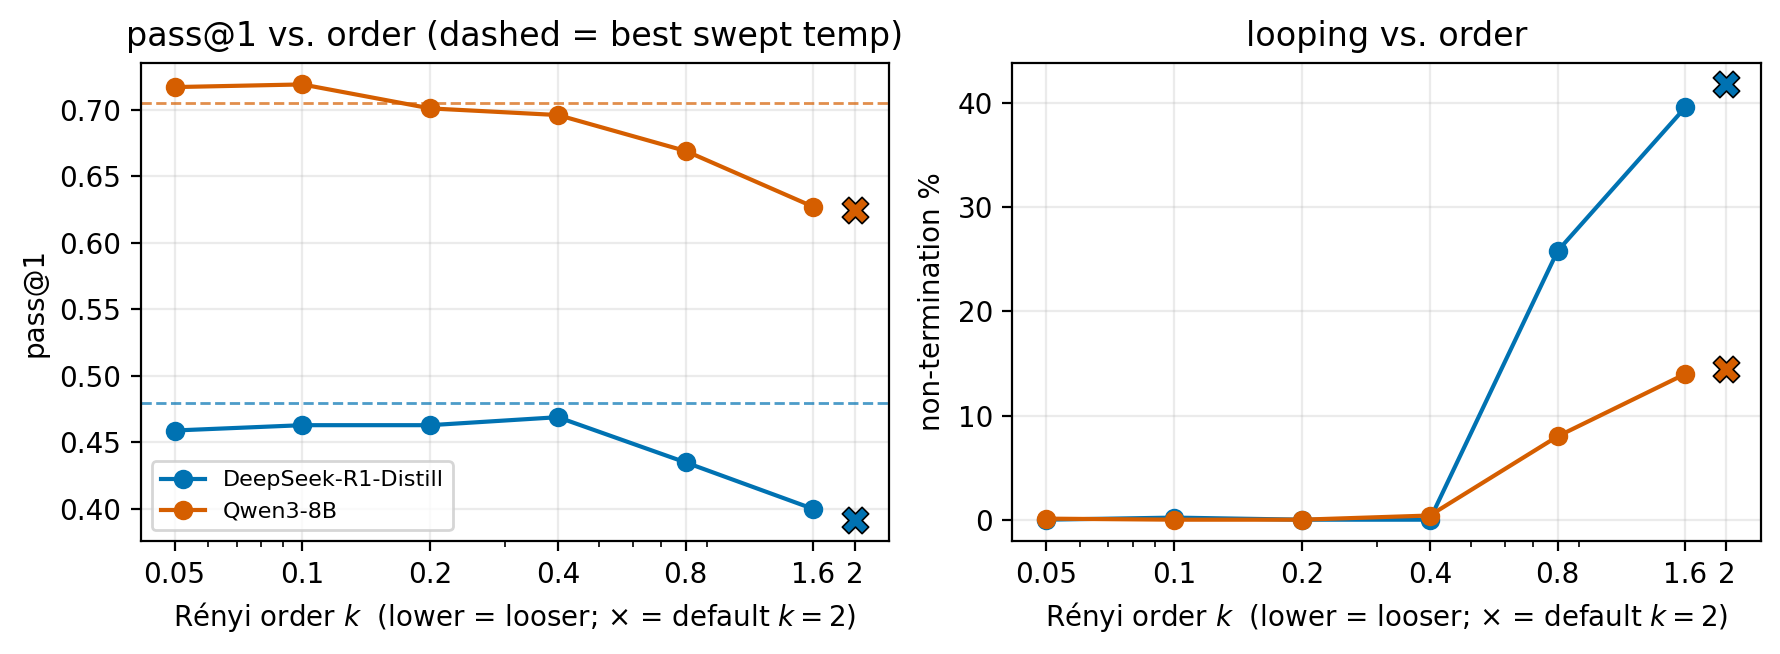
\includegraphics[width=\linewidth]{fig_gk_sweep.png}
\caption{Lowering the R\'enyi order $k$ from the default ($\times$, $k{=}2$) recovers pass@1 (left) and
collapses looping (right). Dashed lines mark each model's best swept temperature: Qwen's $G_k$ curve
rises \emph{above} it (an outright win), DeepSeek's stays just below (a competitive repair).}
\label{fig:gk}
\end{figure}

\paragraph{Token efficiency tracks the loop rate.} Because the savings come from not spending budget on
loops, the token advantage scales with how much the model loops (Table~\ref{tab:main}). On DeepSeek
(heavy looper), $G_k{=}0.4$ is the most token-efficient decoder we test---$9.6$k thinking tokens, fewer
than the recommended ($9.9$k) and swept ($9.7$k) temperatures---at comparable pass@1, and not via
truncation ($0\%$ non-termination). On Qwen (light looper) it is a tie ($\sim$10.8k, indistinguishable
from temperature). We therefore do not claim $G_k$ is universally more token-efficient; the edge is
loop-rate-dependent.

Setting a looser order up front (prevention) also beats detecting and chopping the loop reactively:
prevention ($k{=}0.4$) reaches $0.469$ on DeepSeek versus $0.457$ for adaptive chop-and-continue, and
ties on Qwen---the flatter survivor set suppresses re-entry into the loop after a chop, where $k{=}2$
re-enters.

\subsection{Attributing the gain}\label{sec:ablation}
Does lowering $k$ help by escaping the loops, or for an unrelated reason---say a rich-get-richer effect
that just polishes easy problems? We test this per problem, paired against the $k{=}2$ default on the
same 252 problems (we compare per-problem pass \emph{rates}, since samples are independent across
configs; full tables and limitations in Appendix~\ref{app:ablation}). Three findings.

\textbf{The gain is broad, not a few outliers.} Far more problems improve than regress (Qwen $105$
vs.\ $19$ at $k{=}0.1$; DeepSeek $108$ vs.\ $36$ at $k{=}0.4$), and the mean per-problem $\Delta$pass@1
is well clear of zero: Qwen $+0.094$ ($95\%$ CI $[+0.067,+0.121]$), DeepSeek $+0.077$
($[+0.049,+0.106]$)---both two-level bootstrap intervals exclude 0.

\textbf{It lands on the borderline problems.} Grouping problems by their default difficulty, the gain
concentrates on the mid- and hard-difficulty ones; already-solved problems stay solved and never-solved
ones stay unsolved. Loosening does not simply reward what was already easy---so this is not a
rich-get-richer effect.

\textbf{It is loop-escape.} A problem's gain tracks how much it was truncating at $k{=}2$, and we can
\emph{bound} the effect rather than merely correlate: only a de-truncated sample can be rescued, so
loop-escape explains at most the drop in truncation. That ceiling still leaves \emph{at least $22\%$}
of Qwen's mid-difficulty gain as genuine, non-loop improvement; on DeepSeek, where $68.8\%$ of default
failures are loops, it permits the gain to be almost entirely loop-escape.

The two models differ in \emph{kind}. Qwen's gain is \textbf{reliability}: pass@10 barely moves
($95\%$ CI $[-0.004,+0.056]$, spanning 0), so loosening just makes borderline solutions land more
often. DeepSeek's is \textbf{coverage}: pass@10 rises $+0.10$ ($[+0.056,+0.143]$, excluding 0) and $28$
problems become solvable that never were---their defaults had failed by looping, not by inability.

\section{Positioning}\label{sec:pos}
\paragraph{$G_k$ vs.\ what a practitioner would actually run.} The right baseline is not a swept
temperature but the setting a user gets out of the box, and the picture is model-dependent
(Table~\ref{tab:pos}). On Qwen, $G_k{=}0.1$ ($0.719$) has the best pass@1 of any decoder we test---above
the recommended $T0.6/p0.95/k20$ ($0.680$) \emph{and} above the best hand-swept temperature (pure
temperature $T1.0$: $0.712$; App~\ref{app:topp}), which edges $G_k$ only on pass@10 ($0.849$ vs.\
$0.845$)---a calibration-free win on the headline metric. On DeepSeek, lowering $k$ repairs the catastrophic default ($0.392\!\to\!0.469$)
and leads the recommended setting on pass@10, thinking tokens, and non-termination, but trails it on
pass@1 ($0.469$ vs.\ $0.475$) and the swept temperature ($0.480$). So $G_k$ is a competitive,
calibration-free repair---outright best on the lighter looper, and on the heavier looper a fix that
closes most of the gap to a tuned temperature with no tuning.

\begin{table}[t]\centering
\caption{\textbf{pass@1} for the comparison that matters for a hyperparameter-free method: no-tuning
options vs.\ a tuned one (\textbf{bold} = best in row). On Qwen, $G_k$ (no tuning) beats even the swept
temperature; on DeepSeek it repairs the default but trails the recommended and swept temperatures.}
\label{tab:pos}
\begin{tabular}{lccc}
\toprule
Model & $G_k$ (no tune) & recommended (no tune) & best swept temp \\
\midrule
DeepSeek-R1-Distill & $k{=}0.4$: 0.469 & 0.475 & \textbf{0.480} \\
Qwen3-8B            & $k{=}0.1$: \textbf{0.719} & 0.680 & 0.712 \\
\bottomrule
\end{tabular}
\end{table}

\section{Discussion and Limitations}\label{sec:disc}
The study covers two 8B reasoning models and one benchmark (APPS); whether the mechanism and the
$G_k$ lever transfer to other model families and code benchmarks is open. $G_k$ is the single best
decoder on Qwen but trails a hand-swept temperature on DeepSeek, so this is a diagnosis-and-repair
result, not a uniform decoding win.
We characterize the failure as a per-step collapse of the survivor set toward the most-probable token
and do not benchmark greedy decoding itself, so we do not claim p-less reproduces greedy's
sequence-level behavior; the model-side origin of the looping propensity we take as given (\S\ref{sec:mech}).

\section{Conclusion}\label{sec:conc}
Hyperparameter-free is not assumption-free. On the peaked distributions of reasoning-model
chain-of-thought, a collision-probability threshold silently collapses its survivor set to the single
most-probable token, driving up to 42\% of code traces into loops---amplifying these reasoning models'
latent, training-induced loop-propensity rather than creating it, by removing the sampling diversity
that lets temperature escape. Lowering the R\'enyi order of the same threshold---the origin paper's own
proposed generalization, which we are first to evaluate---repairs the failure and is competitive out of
the box (the best pass@1 on one of our two models). The lesson is that a hyperparameter-free
default can fail silently on a setting its designers never tested, and that the fix can be the design's
own, previously un-evaluated, generalization.

\bibliographystyle{plainnat}
\bibliography{refs}

\appendix
\section{Per-problem ablation: full decomposition}\label{app:ablation}
\paragraph{Design.} For each model we pair every $G_k$ arm against the $k{=}2$ default over the same
252 problems and compare per-problem pass \emph{rates} (samples are independent draws across configs,
so individual samples are not tracked). pass@1 is $c/n$ per problem; pass@10 with $n{=}10$ is the
solved-at-least-once indicator. Significance is read from \emph{two-level bootstrap} $95\%$ CIs on
$\Delta$pass@1 and $\Delta$pass@10---resampling the 252 problems and, within each, the 10 draws for
baseline and arm independently---so the intervals reflect within-problem sampling noise; a CI excluding
0 is a significant shift (Table~\ref{tab:ablation}).

\begin{table}[H]\centering\small
\caption{Per-problem ablation vs.\ the $k{=}2$ default (252 tasks, $n{=}10$). win/lose/net counts
problems whose pass@1 rose/fell; $95\%$ CIs are two-level bootstraps (problems $\times$ draws); a CI
excluding 0 is significant. Note Qwen's $\Delta$pass@10 CIs all span 0 (reliability, not new coverage),
while DeepSeek's exclude 0 (genuine coverage).}
\label{tab:ablation}
\begin{tabular}{lccccc}
\toprule
$k$ & pass@1 ($\Delta$) & pass@10 ($\Delta$) & win/lose/net & $\Delta$pass@1 95\% CI & $\Delta$pass@10 95\% CI \\
\midrule
\multicolumn{6}{l}{\textit{DeepSeek-R1-Distill-Llama-8B}}\\
1.6  & 0.400 ($+$0.008) & 0.643 ($+$0.016) & 66/50/$+$16 & $[-0.015,+0.031]$ & $[-0.024,+0.060]$ \\
0.8  & 0.435 ($+$0.042) & 0.687 ($+$0.060) & 83/44/$+$39 & $[+0.017,+0.069]$ & $[+0.020,+0.107]$ \\
0.4  & 0.469 ($+$0.077) & 0.730 ($+$0.103) & 108/36/$+$72 & $[+0.049,+0.106]$ & $[+0.056,+0.143]$ \\
0.2  & 0.463 ($+$0.071) & 0.730 ($+$0.103) & 100/36/$+$64 & $[+0.043,+0.100]$ & $[+0.056,+0.143]$ \\
0.1  & 0.463 ($+$0.070) & 0.714 ($+$0.087) & 99/32/$+$67 & $[+0.042,+0.099]$ & $[+0.048,+0.131]$ \\
0.05 & 0.459 ($+$0.066) & 0.710 ($+$0.083) & 96/35/$+$61 & $[+0.039,+0.093]$ & $[+0.040,+0.131]$ \\
\midrule
\multicolumn{6}{l}{\textit{Qwen3-8B}}\\
1.6  & 0.627 ($+$0.001) & 0.813 ($-$0.012) & 62/53/$+$9  & $[-0.021,+0.023]$ & $[-0.036,+0.020]$ \\
0.8  & 0.669 ($+$0.044) & 0.837 ($+$0.012) & 83/37/$+$46 & $[+0.021,+0.068]$ & $[-0.012,+0.044]$ \\
0.4  & 0.696 ($+$0.070) & 0.833 ($+$0.008) & 89/30/$+$59 & $[+0.045,+0.096]$ & $[-0.012,+0.048]$ \\
0.2  & 0.701 ($+$0.076) & 0.833 ($+$0.008) & 95/25/$+$70 & $[+0.049,+0.103]$ & $[-0.012,+0.044]$ \\
0.1  & 0.719 ($+$0.094) & 0.845 ($+$0.020) & 105/19/$+$86 & $[+0.067,+0.121]$ & $[-0.004,+0.056]$ \\
0.05 & 0.717 ($+$0.091) & 0.833 ($+$0.008) & 99/22/$+$77 & $[+0.065,+0.119]$ & $[-0.008,+0.044]$ \\
\bottomrule
\end{tabular}
\end{table}

\paragraph{Where the gain lands (strata).} Binning problems by their $k{=}2$ pass@1 into dead ($0$),
hard $(0,0.3]$, mid $(0.3,0.7]$, easy $(0.7,1]$, the mean $\Delta$pass@1 at each model's optimum
concentrates in the mid/hard bins (Qwen $k{=}0.1$: mid $+0.257$, hard $+0.221$; dead $+0.043$, easy
$+0.026$. DeepSeek $k{=}0.4$: hard $+0.175$, mid $+0.144$, dead $+0.073$, easy $-0.020$). Already-solved
(easy) problems barely move and never-solved (dead) mostly stay dead---the gain is not rich-get-richer.
The dominant migration is mid$\to$easy (Qwen $k{=}0.1$: 31 of 47 mid problems).

\paragraph{Loop-escape bound (the rigorous attribution).} Within each stratum we record how far
truncation fell from $k{=}2$ ($\Delta$trunc). Because only a de-truncated sample can be rescued,
loop-escape explains \emph{at most} $|\Delta$trunc$|$ of the pass-rate gain---a problem-level ceiling
(samples are unpaired across configs, so this bounds the loop contribution rather than tracing
individual samples). On Qwen's mid stratum at
$k{=}0.1$, $\Delta$pass@1 $=+0.257$ while truncation fell only $0.20$, so
$\ge(0.257{-}0.20)/0.257\approx22\%$ of that gain is genuine non-loop improvement. On DeepSeek,
$68.8\%$ of default failing samples are truncated loops and truncation falls to $0$ in every stratum,
so the bound is consistent with the gain being predominantly loop-escape. (A coarser per-problem
heuristic agrees directionally but over-credits loops; we report the bound.)

\paragraph{Reliability vs.\ coverage.} On Qwen pass@10 is statistically flat across $k$ ($+0.02$ at the
optimum; $95\%$ CI $[-0.004,+0.056]$, spanning 0): the gain is \emph{reliability}---borderline solutions
land more often. On DeepSeek pass@10 rises $+0.10$ ($[+0.056,+0.143]$, excluding 0) and $28$ never-solved
problems become solvable at $k{=}0.4$: the gain includes genuine \emph{coverage}, because those defaults
failed by looping, not inability.

\section{Full pass@\texorpdfstring{$k$}{k} and cover@\texorpdfstring{$t$}{t}}\label{app:passk}
For completeness we report the full pass@$k$ curve and cover@$t$ for the Table~\ref{tab:main} config
set, both models---recomputed from the same runs (pass@1 and pass@10 match Table~\ref{tab:main}
exactly). pass@$k$ (Table~\ref{tab:passk}) rises monotonically in $k$; the decoder ordering is broadly
stable, though on Qwen $G_k{=}0.1$ leads at pass@1 while the unfiltered temperature leads from pass@5
up---the reliability-vs-coverage distinction of \S\ref{sec:ablation}. cover@$t$ (Table~\ref{tab:cover})
is the fraction of problems solved on at least a fraction $t$ of the $n{=}10$ samples (a
\emph{reliability} measure), and its distinct variant requires $\ge tn$ AST-\emph{distinct} correct
solutions (a solution-\emph{diversity} measure; $\le$ cover@$t$ by construction). Both rise sharply as
$k$ falls---e.g.\ Qwen cover@$0.7$ goes $58.3\%\!\to\!71.4\%$ (default $\to$ $G_k{=}0.1$) and its
distinct form $44.0\%\!\to\!64.3\%$---so lowering the order makes problems solved both more
\emph{consistently} and with more \emph{distinct} correct programs.

\begin{table}[H]\centering\small
\caption{Full pass@$k$ (APPS-interview, $n{=}10$, thinking on), recomputed from the same runs as
Table~\ref{tab:main} (unbiased estimator; pass@1/@10 match Table~\ref{tab:main}). $^\dagger$ = strongest
swept temperature.}
\label{tab:passk}
\begin{tabular}{lccccc}
\toprule
Config & pass@1 & pass@3 & pass@5 & pass@8 & pass@10 \\
\midrule
\multicolumn{6}{l}{\textit{DeepSeek-R1-Distill-Llama-8B}}\\
p-less $k{=}2$ (default) & 0.392 & 0.527 & 0.574 & 0.611 & 0.627 \\
p-less-norm (default) & 0.392 & 0.533 & 0.590 & 0.640 & 0.663 \\
$G_k{=}1.6$ & 0.400 & 0.542 & 0.592 & 0.629 & 0.643 \\
$G_k{=}0.8$ & 0.435 & 0.588 & 0.638 & 0.673 & 0.687 \\
$G_k{=}0.4$ & 0.469 & 0.617 & 0.668 & 0.711 & 0.730 \\
$G_k{=}0.2$ & 0.463 & 0.619 & 0.669 & 0.711 & 0.730 \\
$G_k{=}0.1$ & 0.463 & 0.614 & 0.663 & 0.699 & 0.714 \\
$G_k{=}0.05$ & 0.459 & 0.608 & 0.657 & 0.695 & 0.710 \\
temp $T{=}0.6,p0.95$ (rec) & 0.475 & 0.612 & 0.657 & 0.696 & 0.714 \\
temp $T{=}1.0$ (unfilt) $^\dagger$ & 0.451 & 0.595 & 0.637 & 0.667 & 0.679 \\
\midrule
\multicolumn{6}{l}{\textit{Qwen3-8B}}\\
p-less $k{=}2$ (default) & 0.625 & 0.757 & 0.792 & 0.815 & 0.825 \\
p-less-norm (default) & 0.629 & 0.755 & 0.791 & 0.817 & 0.829 \\
$G_k{=}1.6$ & 0.627 & 0.751 & 0.786 & 0.807 & 0.813 \\
$G_k{=}0.8$ & 0.669 & 0.779 & 0.808 & 0.829 & 0.837 \\
$G_k{=}0.4$ & 0.696 & 0.788 & 0.811 & 0.828 & 0.833 \\
$G_k{=}0.2$ & 0.701 & 0.788 & 0.811 & 0.827 & 0.833 \\
$G_k{=}0.1$ & 0.719 & 0.796 & 0.818 & 0.837 & 0.845 \\
$G_k{=}0.05$ & 0.717 & 0.798 & 0.815 & 0.828 & 0.833 \\
temp $T{=}0.6,p0.95,k20$ (rec) & 0.680 & 0.777 & 0.804 & 0.822 & 0.829 \\
temp $T{=}1.0$ (unfilt) $^\dagger$ & 0.712 & 0.801 & 0.824 & 0.841 & 0.849 \\
\bottomrule
\end{tabular}
\end{table}

\begin{table}[H]\centering\small
\caption{cover@$t$ (\% of problems solved on $\ge t$ of the $n{=}10$ samples) and its distinct variant
cover@$t$-d (\% with $\ge tn$ AST-\emph{distinct} correct solutions). Same runs / config set as
Table~\ref{tab:main}; cover@$t$-d $\le$ cover@$t$ always. cover@$0.1$ equals pass@10 and is omitted.}
\label{tab:cover}
\begin{tabular}{lcccccc}
\toprule
Config & cov@.3 & cov@.5 & cov@.7 & cov@.3-d & cov@.5-d & cov@.7-d \\
\midrule
\multicolumn{7}{l}{\textit{DeepSeek-R1-Distill-Llama-8B}}\\
p-less $k{=}2$ (default) & 50.0 & 42.9 & 32.9 & 48.8 & 38.5 & 27.0 \\
p-less-norm (default) & 48.8 & 40.9 & 34.9 & 47.2 & 38.5 & 25.8 \\
$G_k{=}1.6$ & 51.6 & 41.3 & 33.7 & 48.8 & 37.3 & 27.0 \\
$G_k{=}0.8$ & 56.0 & 48.4 & 36.9 & 54.4 & 44.8 & 30.2 \\
$G_k{=}0.4$ & 59.5 & 50.4 & 43.3 & 58.7 & 49.2 & 38.5 \\
$G_k{=}0.2$ & 58.3 & 52.0 & 40.9 & 57.5 & 50.8 & 37.7 \\
$G_k{=}0.1$ & 58.7 & 50.4 & 41.3 & 57.9 & 48.8 & 37.7 \\
$G_k{=}0.05$ & 57.1 & 50.4 & 40.5 & 56.3 & 49.2 & 36.5 \\
temp $T{=}0.6,p0.95$ (rec) & 57.5 & 52.8 & 42.9 & 56.7 & 49.2 & 36.1 \\
temp $T{=}1.0$ (unfilt) $^\dagger$ & 57.5 & 50.0 & 40.9 & 56.3 & 48.4 & 38.1 \\
\midrule
\multicolumn{7}{l}{\textit{Qwen3-8B}}\\
p-less $k{=}2$ (default) & 75.4 & 67.1 & 58.3 & 73.4 & 60.3 & 44.0 \\
p-less-norm (default) & 73.8 & 67.1 & 59.5 & 71.8 & 61.9 & 46.8 \\
$G_k{=}1.6$ & 75.8 & 65.9 & 58.3 & 73.4 & 59.9 & 44.8 \\
$G_k{=}0.8$ & 76.6 & 71.8 & 64.7 & 74.2 & 65.9 & 54.0 \\
$G_k{=}0.4$ & 77.4 & 73.8 & 66.7 & 74.6 & 67.9 & 55.6 \\
$G_k{=}0.2$ & 77.8 & 73.8 & 68.7 & 75.8 & 69.4 & 61.5 \\
$G_k{=}0.1$ & 77.8 & 75.0 & 71.4 & 77.0 & 71.4 & 64.3 \\
$G_k{=}0.05$ & 79.4 & 76.6 & 69.8 & 77.4 & 71.8 & 61.9 \\
temp $T{=}0.6,p0.95,k20$ (rec) & 77.0 & 71.4 & 64.3 & 75.8 & 66.7 & 53.6 \\
temp $T{=}1.0$ (unfilt) $^\dagger$ & 79.4 & 74.2 & 67.9 & 78.6 & 69.8 & 58.7 \\
\bottomrule
\end{tabular}
\end{table}

\section{Top-p (nucleus) sampling: a comparison}\label{app:topp}
As a baseline for the R\'enyi-order lever, we sweep temperature-$1.0$ nucleus sampling at
$p\in\{0.8,0.85,0.9,1.0\}$ ($p{=}1.0$ is pure temperature, no truncation), on the same footing as the
$G_k$ sweep (vLLM, 252 problems, $n{=}10$, thinking on, $32{,}768$-token cap; Table~\ref{tab:topp}). The
question is whether plain nucleus sampling reaches what lowering the R\'enyi order $k$ achieves.

\begin{table}[H]\centering\small
\caption{Top-p (nucleus) sweep at $T{=}1.0$ (APPS-interview, $n{=}10$, thinking on). cb\_div is
correct-only and not comparable across configs (\S\ref{sec:setup}).}
\label{tab:topp}
\begin{tabular}{lccccc}
\toprule
Config & pass@1 & pass@10 & cb\_div & mean think tok & non-term \% \\
\midrule
\multicolumn{6}{l}{\textit{DeepSeek-R1-Distill-Llama-8B}}\\
top-p 0.8             & 0.465 & 0.726 & 0.541 & 9{,}085 & 0.6 \\
top-p 0.85            & 0.480 & 0.722 & 0.558 & 9{,}251 & 0.0 \\
top-p 0.9             & 0.480 & 0.726 & 0.562 & 9{,}216 & 0.0 \\
top-p 1.0 (pure temp) & 0.451 & 0.679 & 0.588 & 9{,}770 & 0.0 \\
\midrule
\multicolumn{6}{l}{\textit{Qwen3-8B}}\\
top-p 0.8             & 0.700 & 0.841 & 0.478 & 10{,}679 & 0.8 \\
top-p 0.85            & 0.699 & 0.841 & 0.476 & 10{,}943 & 0.4 \\
top-p 0.9             & 0.706 & 0.841 & 0.491 & 10{,}778 & 0.2 \\
top-p 1.0 (pure temp) & 0.712 & 0.849 & 0.503 & 10{,}738 & 0.0 \\
\bottomrule
\end{tabular}
\end{table}

\paragraph{Can nucleus sampling match $G_k$?} It depends on the model. On \textbf{DeepSeek}, yes:
top-p $0.85$/$0.9$ ($0.480$ pass@1) ties the best temperature and edges $G_k{=}0.4$ ($0.469$)---on the
heavier looper, plain nucleus sampling is as good a repair as the R\'enyi-order lever. On
\textbf{Qwen}, not on the headline metric: the best top-p is pure temperature ($p{=}1.0$, $0.712$),
which $G_k{=}0.1$ ($0.719$) still exceeds on pass@1; on pass@10 the two are within noise ($0.845$ vs.\
$0.849$). Two things hold across the sweep: every top-p arm terminates ($\le0.8\%$ non-termination),
re-confirming that the looping failure is specific to the p-less threshold and not the
temperature/nucleus family; and for Qwen \emph{looser} nucleus is better (pass@1 rises monotonically to
$p{=}1.0$), so nucleus truncation does not help.

\end{document}
